% ============================================================================
% FOOTBALL CLUB MANAGEMENT SYSTEM — PROJECT REPORT
% Academic LaTeX Report — April 2026
% ============================================================================
\documentclass[12pt,a4paper,oneside]{report}

% ── Encoding & Fonts ────────────────────────────────────────────────────────
\usepackage[utf8]{inputenc}
\usepackage[T1]{fontenc}
\usepackage{mathptmx}               % Times New Roman clone
\usepackage{setspace}
\onehalfspacing                      % 1.5 line spacing

% ── Page Geometry ───────────────────────────────────────────────────────────
\usepackage[
  top=1in, bottom=1in,
  left=1.25in, right=1in
]{geometry}

% ── Graphics, Tables, Colors ───────────────────────────────────────────────
\usepackage{graphicx}
\usepackage{xcolor}
\usepackage{booktabs}
\usepackage{tabularx}
\usepackage{longtable}
\usepackage{array}
\usepackage{multirow}
\usepackage{colortbl}
\usepackage{float}
\usepackage{caption}
\usepackage{subcaption}

% ── TikZ for Diagrams ──────────────────────────────────────────────────────
\usepackage{tikz}
\usetikzlibrary{shapes.geometric, arrows.meta, positioning, calc, fit, backgrounds}

% ── Listings (code snippets) ──────────────────────────────────────────────
\usepackage{listings}
\lstset{
  basicstyle=\ttfamily\small,
  breaklines=true,
  frame=single,
  backgroundcolor=\color{gray!5},
  keywordstyle=\color{blue!70!black},
  commentstyle=\color{green!50!black},
  stringstyle=\color{red!60!black},
  showstringspaces=false
}

% ── Hyperlinks ──────────────────────────────────────────────────────────────
\usepackage[
  colorlinks=true,
  linkcolor=black,
  citecolor=blue!60!black,
  urlcolor=blue!60!black
]{hyperref}

% ── Headers / Footers ──────────────────────────────────────────────────────
\usepackage{fancyhdr}
\pagestyle{fancy}
\fancyhf{}
\fancyhead[L]{\small\leftmark}
\fancyhead[R]{\small Football Club Management System}
\fancyfoot[C]{\thepage}
\renewcommand{\headrulewidth}{0.4pt}
\renewcommand{\footrulewidth}{0pt}

% ── Chapter/Section Formatting ──────────────────────────────────────────────
\usepackage{titlesec}
\titleformat{\chapter}[display]
  {\normalfont\Large\bfseries\centering}
  {\MakeUppercase{\chaptertitlename}\ \thechapter}{12pt}{\LARGE\MakeUppercase}
\titlespacing*{\chapter}{0pt}{-20pt}{24pt}

\titleformat{\section}
  {\normalfont\large\bfseries}{\thesection}{1em}{}
\titleformat{\subsection}
  {\normalfont\normalsize\bfseries}{\thesubsection}{1em}{}

% ── Bibliography ────────────────────────────────────────────────────────────
\usepackage[numbers,sort&compress]{natbib}

% ── Misc ────────────────────────────────────────────────────────────────────
\usepackage{enumitem}
\usepackage{parskip}
\usepackage{pdfpages}

% ── Custom Colors ───────────────────────────────────────────────────────────
\definecolor{fcRed}{RGB}{200,16,46}
\definecolor{darkBg}{RGB}{10,10,24}
\definecolor{accentGold}{RGB}{218,165,32}
\definecolor{tableHeader}{RGB}{44,62,80}
\definecolor{tableRow}{RGB}{245,247,250}

% ── DFD Styles ──────────────────────────────────────────────────────────────
\tikzstyle{entity}   = [rectangle, draw, fill=blue!8, text centered,
                         minimum height=1cm, minimum width=2.2cm,
                         font=\small\bfseries, rounded corners=2pt]
\tikzstyle{process}  = [circle, draw, fill=orange!10, text centered,
                         minimum size=1.6cm, font=\scriptsize\bfseries,
                         text width=1.3cm, align=center]
\tikzstyle{datastore}= [rectangle split, rectangle split parts=2,
                         draw, fill=green!6, text centered,
                         font=\scriptsize, minimum width=2.2cm]
\tikzstyle{arrow}    = [-{Stealth[length=2.5mm]}, thick]

% ── Title-page variables ───────────────────────────────────────────────────
\newcommand{\projecttitle}{FOOTBALL CLUB MANAGEMENT SYSTEM}
\newcommand{\projectsubtitle}{A Comprehensive Web-Based Solution for\\
  Digitizing Football Club Operations}
\newcommand{\reportdate}{April 2026}

% ============================================================================
\begin{document}

% ────────────────────────────────────────────────────────────────────────────
%  TITLE PAGE
% ────────────────────────────────────────────────────────────────────────────
\begin{titlepage}
  \centering
  \vspace*{1.5cm}

  {\Huge\bfseries PROJECT REPORT\par}
  \vspace{0.6cm}
  {\Large on\par}
  \vspace{0.6cm}
  {\Huge\bfseries\color{fcRed} \projecttitle\par}
  \vspace{0.4cm}
  {\large\itshape \projectsubtitle\par}

  \vspace{1.2cm}
  \rule{0.6\textwidth}{0.5pt}
  \vspace{0.8cm}

  {\large\textbf{Submitted in partial fulfillment of the requirements}\\
  \textbf{for the award of the Degree of}\\[6pt]
  \textbf{Bachelor of Computer Applications (BCA)}\par}

  \vspace{1cm}

  {\large\textbf{Submitted by:}\par}
  \vspace{0.3cm}
  {\Large Athul\par}

  \vspace{0.8cm}

  {\large\textbf{Under the guidance of:}\par}
  \vspace{0.3cm}
  {\Large Faculty Guide\par}

  \vfill

  {\large
    \textbf{Department of Computer Applications}\\[4pt]
    University Name\\[4pt]
    \reportdate
  \par}
\end{titlepage}

% ────────────────────────────────────────────────────────────────────────────
%  CERTIFICATE PAGE
% ────────────────────────────────────────────────────────────────────────────
\newpage
\thispagestyle{empty}
\begin{center}
  {\Large\bfseries CERTIFICATE}\\[24pt]
\end{center}

This is to certify that the project report entitled \textbf{``Football Club Management System''} submitted by \textbf{Athul} is a bonafide record of the project work carried out under my guidance and supervision in partial fulfillment of the requirements for the award of the degree of \textbf{Bachelor of Computer Applications (BCA)}.

\vspace{2cm}

\noindent
\begin{minipage}[t]{0.45\textwidth}
  \centering
  \rule{5cm}{0.4pt}\\[4pt]
  \textbf{Internal Guide}\\
  Department of Computer Applications
\end{minipage}
\hfill
\begin{minipage}[t]{0.45\textwidth}
  \centering
  \rule{5cm}{0.4pt}\\[4pt]
  \textbf{Head of Department}\\
  Department of Computer Applications
\end{minipage}

\vspace{2.5cm}
\noindent
\begin{minipage}[t]{0.45\textwidth}
  \centering
  \rule{5cm}{0.4pt}\\[4pt]
  \textbf{External Examiner}
\end{minipage}

\vspace{1.5cm}
\noindent\textbf{Date:} \hspace{2cm} \textbf{Place:}

% ────────────────────────────────────────────────────────────────────────────
%  DECLARATION
% ────────────────────────────────────────────────────────────────────────────
\newpage
\thispagestyle{empty}
\begin{center}
  {\Large\bfseries DECLARATION}\\[24pt]
\end{center}

I hereby declare that the project report entitled \textbf{``Football Club Management System''} is an authentic record of my own work carried out as a requirement for the award of the degree of \textbf{Bachelor of Computer Applications (BCA)}. This work has not been submitted to any other university or institution for the award of any degree or diploma.

\vspace{2cm}

\noindent
\begin{flushright}
  \rule{5cm}{0.4pt}\\[4pt]
  \textbf{Athul}\\
  Date: \reportdate
\end{flushright}

% ────────────────────────────────────────────────────────────────────────────
%  ACKNOWLEDGEMENT
% ────────────────────────────────────────────────────────────────────────────
\newpage
\thispagestyle{empty}
\begin{center}
  {\Large\bfseries ACKNOWLEDGEMENT}\\[24pt]
\end{center}

I would like to express my sincere gratitude to all those who contributed to the successful completion of this project.

I am deeply grateful to my project guide for the continuous support, invaluable guidance, and constructive feedback provided throughout the development of this project. The technical insights and mentorship were instrumental in shaping the system architecture and feature set.

I extend my heartfelt thanks to the \textbf{Head of the Department of Computer Applications} for providing the necessary infrastructure and academic environment that facilitated this work.

I also wish to thank the staff members and fellow students who participated in the User Acceptance Testing phase, providing the practical feedback that helped refine the system's usability and functionality.

Finally, I express my gratitude to my family and friends for their unwavering encouragement and moral support throughout the duration of this project.

\vspace{1.5cm}
\begin{flushright}
  \textbf{Athul}
\end{flushright}

% ────────────────────────────────────────────────────────────────────────────
%  ABSTRACT
% ────────────────────────────────────────────────────────────────────────────
\newpage
\thispagestyle{empty}
\begin{center}
  {\Large\bfseries ABSTRACT}\\[24pt]
\end{center}

The \textbf{Football Club Management System} is a comprehensive, full-stack web application built on the MERN stack (MongoDB, Express.js, React.js, Node.js) designed to digitize and streamline every operational facet of a professional football club. Traditional football club management relies on fragmented manual processes---spreadsheets for player statistics, paper forms for leave requests, phone calls for training notifications, and disconnected filing cabinets for contracts. This project replaces that paradigm with a centralized, real-time, role-based digital platform.

The system provides four distinct, interconnected dashboards for \textbf{Admin}, \textbf{Manager}, \textbf{Coach}, and \textbf{Player} roles, each equipped with tailored tools and live data powered by Socket.IO WebSocket communication. Key capabilities include user lifecycle management with immutable audit logging, fixture scheduling with tactical lineup building, training session management with attendance tracking, squad health monitoring with injury and fitness tracking, leave request workflows with real-time approval notifications, document vault with OCR scanning, and equipment inventory management.

Beyond standard CRUD operations, the application integrates four AI-powered features: an OCR document scanner, an AI chatbot, a document preparation assistant, and a text summarization engine. The system employs enterprise-grade security through JWT authentication, bcrypt password hashing, Helmet security headers, CORS policies, multi-tier rate limiting, and input sanitization. The cinematic, EA FC-inspired user interface features dark-mode glassmorphism, animated player cards, and dynamic page transitions.

The system was developed, tested through unit, integration, and user acceptance testing, and validated against 25 formal test cases---all passing successfully.

\vspace{0.5cm}
\noindent\textbf{Keywords:} MERN Stack, Football Club Management, Real-Time Communication, Socket.IO, Role-Based Access Control, AI Integration, MongoDB, React.js, Node.js

% ────────────────────────────────────────────────────────────────────────────
%  TABLE OF CONTENTS, LIST OF FIGURES, LIST OF TABLES
% ────────────────────────────────────────────────────────────────────────────
\newpage
\tableofcontents

\newpage
\listoffigures

\newpage
\listoftables

% ────────────────────────────────────────────────────────────────────────────
%  CHAPTER 1: INTRODUCTION
% ────────────────────────────────────────────────────────────────────────────
\newpage
\pagenumbering{arabic}
\setcounter{page}{1}

\chapter{INTRODUCTION}

\section{Project Overview}

The Football Club Management System is a comprehensive, web-based application designed to replace traditional, paper-based football club operations. It digitizes and streamlines key operational and administrative workflows by providing four distinct, role-based interfaces: an \textbf{Admin Panel} for central control, a \textbf{Manager Panel} for scheduling and resources, a \textbf{Coach Panel} for tactical and squad management, and a \textbf{Player Panel} for personal dashboards and requests.

These modules function as a single, interconnected ecosystem built on the MERN stack (MongoDB, Express.js, React.js, Node.js). The system leverages Socket.IO for real-time WebSocket communication, ensuring that actions taken by one user role are instantly reflected for others. For example, when a coach approves a leave request, the player receives an immediate notification on their dashboard without requiring a page refresh.

The platform integrates four AI-powered capabilities---OCR document scanning, AI chatbot assistance, document preparation, and text summarization---to reduce manual labor and accelerate decision-making. Security is implemented through JWT-based authentication, bcrypt password hashing, role-based access control (RBAC), Helmet security headers, CORS policies, rate limiting, input sanitization, and an immutable audit trail.

\section{Problem Statement}

The traditional football club management system is fundamentally inefficient, relying on outdated, manual, and disconnected processes. The core challenges include:

\begin{itemize}[leftmargin=*]
  \item \textbf{Data Fragmentation:} Player statistics, injury records, and contract details are scattered across multiple spreadsheets with no single source of truth, leading to version conflicts and formula errors.
  \item \textbf{Communication Gaps:} Training schedules, match fixtures, and leave decisions are communicated via WhatsApp groups or phone calls, with no formal logging or acknowledgment system.
  \item \textbf{Administrative Overhead:} Coaches maintain paper-based lineup records, manually track training attendance, and physically compile fitness reports---processes that are time-consuming and error-prone.
  \item \textbf{Security Vulnerabilities:} Sensitive player data is stored in unencrypted formats without access controls, creating compliance and accountability risks.
  \item \textbf{No Audit Trail:} There is no mechanism to track who modified which records and when, making it impossible to trace unauthorized changes.
  \item \textbf{Document Management Chaos:} Physical documents are prone to loss and damage, with no OCR or digital search capability.
\end{itemize}

\section{Project Objectives}

The project is guided by the following specific objectives:

\begin{enumerate}[leftmargin=*]
  \item \textbf{Centralized Operations Hub} --- Build a unified web platform where Admin, Manager, Coach, and Player roles access only the tools relevant to their responsibilities.
  \item \textbf{Real-Time Communication} --- Leverage Socket.IO for live notifications, online-presence tracking, and instant data synchronization across all clients.
  \item \textbf{AI-Augmented Workflows} --- Integrate OCR scanning, AI chatbot, document preparation, and text summarization to reduce manual labor.
  \item \textbf{Immutable Audit Trail} --- Log every CREATE, UPDATE, DELETE, and LOGIN action in a tamper-proof system log.
  \item \textbf{Cinematic UI/UX} --- Deliver a visually stunning, EA FC-inspired interface with dark themes, glassmorphism, animated player cards, and page transitions.
  \item \textbf{Comprehensive Player Lifecycle} --- Support players from recruitment through active play to archival with full career snapshot preservation.
  \item \textbf{Enterprise-Grade Security} --- Protect all data with JWT authentication, bcrypt hashing, Helmet headers, CORS, rate limiting, and input sanitization.
\end{enumerate}

\section{Scope of the Project}

The scope encompasses the following functional domains, as summarized in Table~\ref{tab:scope}.

\begin{table}[H]
\centering
\caption{Functional Scope of the System}
\label{tab:scope}
\small
\begin{tabularx}{\textwidth}{|l|X|}
\hline
\rowcolor{tableHeader}\textcolor{white}{\textbf{Domain}} & \textcolor{white}{\textbf{Description}} \\
\hline
Admin Panel     & User CRUD, player archival/reinstatement, club settings, immutable system logs \\
\hline
\rowcolor{tableRow}
Manager Panel   & Fixtures, contracts, document vault with OCR, inventory, finance dashboard \\
\hline
Coach Panel     & Tactical board with lineup builder, training schedule, squad health, discipline, leave approval, performance tracking \\
\hline
\rowcolor{tableRow}
Player Panel    & Personal dashboard, event calendar, leave request submission \\
\hline
AI Features     & OCR scanner, AI chatbot, document preparation, text summarization \\
\hline
\rowcolor{tableRow}
Real-Time       & Socket.IO notifications, online presence, live data synchronization \\
\hline
Security        & JWT auth, bcrypt, Helmet, CORS, rate limiting, sanitization, immutable logs \\
\hline
\end{tabularx}
\end{table}

\noindent\textbf{Out of Scope:} Payment gateway integration, video analysis, native mobile applications, multi-language support, biometric device integration, third-party football data APIs, multi-club/league management, and parent/guardian portals. These are identified as future enhancements.

% ────────────────────────────────────────────────────────────────────────────
%  CHAPTER 2: SYSTEM SPECIFICATIONS
% ────────────────────────────────────────────────────────────────────────────
\chapter{SYSTEM SPECIFICATIONS}

\section{Software Specification}

The system is developed using a three-layer MERN architecture separating the Presentation, Logic, and Data layers. Table~\ref{tab:software} details the software stack.

\begin{table}[H]
\centering
\caption{Software Specification}
\label{tab:software}
\small
\begin{tabularx}{\textwidth}{|l|l|l|X|}
\hline
\rowcolor{tableHeader}
\textcolor{white}{\textbf{Component}} & \textcolor{white}{\textbf{Technology}} & \textcolor{white}{\textbf{Version}} & \textcolor{white}{\textbf{Purpose}} \\
\hline
Frontend        & React.js + Vite            & 18.x  & SPA with component architecture \\
\hline\rowcolor{tableRow}
Routing         & React Router DOM           & 6.x   & Client-side navigation \\
\hline
State Mgmt      & React Context API          & ---   & AuthContext, SocketContext \\
\hline\rowcolor{tableRow}
Styling         & Vanilla CSS + Tokens       & ---   & Design system with custom properties \\
\hline
Typography      & Google Fonts               & ---   & Bebas Neue (headings), Inter (body) \\
\hline\rowcolor{tableRow}
Backend         & Node.js + Express          & 18.x / 4.18.2 & RESTful API server \\
\hline
Database        & MongoDB + Mongoose         & 7.x / 8.0.0   & NoSQL document store with ODM \\
\hline\rowcolor{tableRow}
Auth            & JWT + bcrypt               & 9.0.2 / 5.1.1 & Token auth + password hashing \\
\hline
Real-Time       & Socket.IO                  & 4.6.0 & WebSocket communication \\
\hline\rowcolor{tableRow}
File Upload     & Multer + Sharp             & 1.4.5 / 0.33.0 & Multipart upload + image processing \\
\hline
Security        & Helmet + CORS + Rate Limit & 7.1.0 / 2.8.5 / 7.1.5 & HTTP headers, CORS, throttling \\
\hline\rowcolor{tableRow}
Sanitization    & sanitize-html + validator  & 2.11.0 / 13.11.0 & XSS prevention, input validation \\
\hline
Testing         & Jest + Supertest           & 29.7.0 / 6.3.3 & Unit + integration testing \\
\hline
\end{tabularx}
\end{table}

\section{Hardware Specification}

Table~\ref{tab:hardware} outlines the hardware requirements for the server and client environments.

\begin{table}[H]
\centering
\caption{Hardware Specification}
\label{tab:hardware}
\small
\begin{tabularx}{\textwidth}{|l|X|X|}
\hline
\rowcolor{tableHeader}
\textcolor{white}{\textbf{Component}} & \textcolor{white}{\textbf{Minimum}} & \textcolor{white}{\textbf{Recommended}} \\
\hline
Processor & Intel Core i3 / AMD Ryzen 3        & Intel Core i5 / AMD Ryzen 5 \\
\hline\rowcolor{tableRow}
RAM       & 4 GB                                & 8 GB or higher \\
\hline
Storage   & 10 GB free disk space               & 20 GB SSD \\
\hline\rowcolor{tableRow}
Display   & 1366 $\times$ 768                   & 1920 $\times$ 1080 Full HD \\
\hline
Network   & Broadband Internet                  & Stable 10 Mbps+ \\
\hline\rowcolor{tableRow}
GPU       & Integrated graphics                 & Dedicated GPU for animations \\
\hline
Browser   & Chrome / Edge (latest)              & Chrome / Edge (latest) \\
\hline
\end{tabularx}
\end{table}

% ────────────────────────────────────────────────────────────────────────────
%  CHAPTER 3: SYSTEM ANALYSIS
% ────────────────────────────────────────────────────────────────────────────
\chapter{SYSTEM ANALYSIS}

\section{Existing System}

The existing system for football club management is a collection of traditional, manual, and disconnected processes:

\begin{itemize}[leftmargin=*]
  \item \textbf{Spreadsheet-Based Tracking:} Player statistics, injury records, and contract dates maintained in Excel/Google Sheets, leading to version conflicts and no access control.
  \item \textbf{Paper-Based Documentation:} Contracts and medical certificates stored as physical files, making retrieval slow and prone to loss.
  \item \textbf{Disconnected Communication:} Training schedules communicated via WhatsApp groups with no formal logging or acknowledgment.
  \item \textbf{No Role Separation:} All staff share the same access level, creating security risks.
  \item \textbf{No Audit Trail:} No record of who changed what and when.
  \item \textbf{No AI Assistance:} All document processing is entirely manual.
  \item \textbf{No Real-Time Updates:} Lineup changes and leave approvals require manual notification.
\end{itemize}

\section{Proposed System}

The proposed Football Club Management System addresses every limitation through a centralized, real-time, web-based platform with four interconnected role-based panels. Figure~\ref{fig:architecture} illustrates the system architecture.

\begin{figure}[H]
\centering
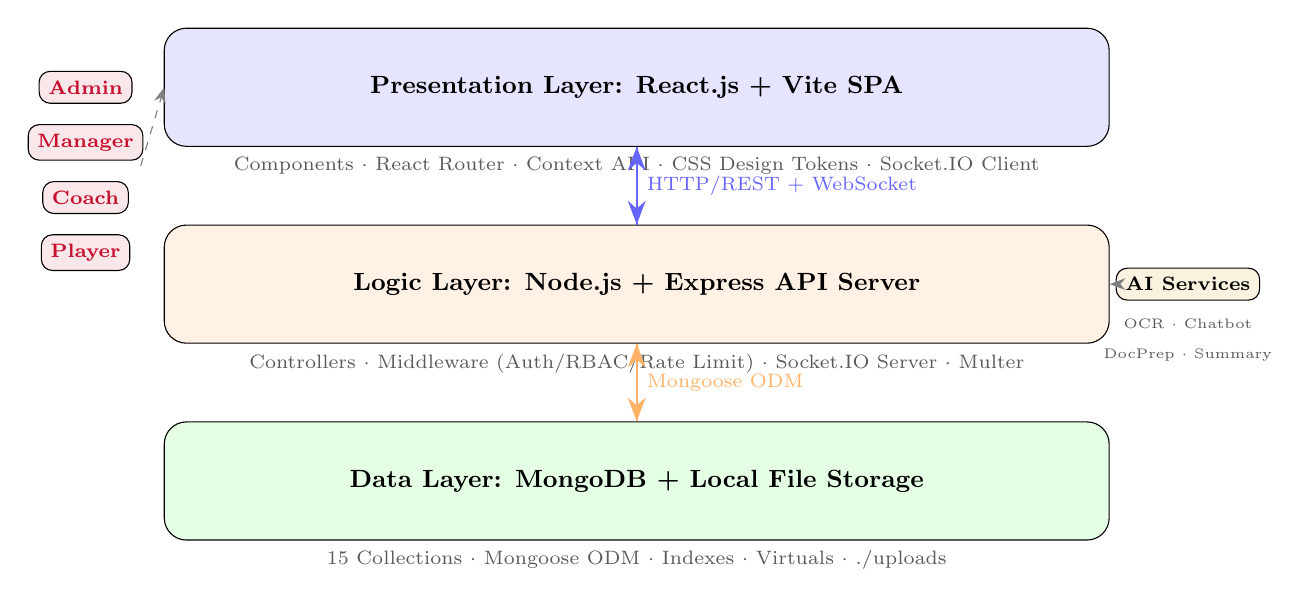
\begin{tikzpicture}[
  layer/.style={draw, rounded corners=8pt, minimum width=12cm, minimum height=1.5cm, text centered, font=\small\bfseries},
  sublabel/.style={font=\scriptsize, text=gray!70!black}
]
% Presentation Layer
\node[layer, fill=blue!10] (client) at (0,6)
  {Presentation Layer: React.js + Vite SPA};
\node[sublabel, below=0pt of client]
  {Components $\cdot$ React Router $\cdot$ Context API $\cdot$ CSS Design Tokens $\cdot$ Socket.IO Client};

% Logic Layer
\node[layer, fill=orange!10] (server) at (0,3.5)
  {Logic Layer: Node.js + Express API Server};
\node[sublabel, below=0pt of server]
  {Controllers $\cdot$ Middleware (Auth/RBAC/Rate Limit) $\cdot$ Socket.IO Server $\cdot$ Multer};

% Data Layer
\node[layer, fill=green!10] (data) at (0,1)
  {Data Layer: MongoDB + Local File Storage};
\node[sublabel, below=0pt of data]
  {15 Collections $\cdot$ Mongoose ODM $\cdot$ Indexes $\cdot$ Virtuals $\cdot$ ./uploads};

% Arrows
\draw[-{Stealth[length=3mm]}, thick, blue!60] (client.south) -- node[right, font=\scriptsize]{HTTP/REST + WebSocket} (server.north);
\draw[-{Stealth[length=3mm]}, thick, blue!60] (server.north) -- (client.south);
\draw[-{Stealth[length=3mm]}, thick, orange!60] (server.south) -- node[right, font=\scriptsize]{Mongoose ODM} (data.north);
\draw[-{Stealth[length=3mm]}, thick, orange!60] (data.north) -- (server.south);

% Side labels for roles
\node[draw, fill=fcRed!10, rounded corners, font=\scriptsize\bfseries, text=fcRed] at (-7,6) {Admin};
\node[draw, fill=fcRed!10, rounded corners, font=\scriptsize\bfseries, text=fcRed] at (-7,5.3) {Manager};
\node[draw, fill=fcRed!10, rounded corners, font=\scriptsize\bfseries, text=fcRed] at (-7,4.6) {Coach};
\node[draw, fill=fcRed!10, rounded corners, font=\scriptsize\bfseries, text=fcRed] at (-7,3.9) {Player};
\draw[-{Stealth[length=2mm]}, dashed, gray] (-6.3,5) -- (-6,6);

% AI label
\node[draw, fill=accentGold!15, rounded corners, font=\scriptsize\bfseries] at (7,3.5) {AI Services};
\node[font=\tiny, text=gray!70!black] at (7,3) {OCR $\cdot$ Chatbot};
\node[font=\tiny, text=gray!70!black] at (7,2.6) {DocPrep $\cdot$ Summary};
\draw[-{Stealth[length=2mm]}, dashed, gray] (6.1,3.5) -- (server.east);

\end{tikzpicture}
\caption{Three-Layer System Architecture}
\label{fig:architecture}
\end{figure}

Key advantages of the proposed system include: a single source of truth for all club data, enterprise-grade security, AI-powered automation, real-time communication via WebSocket, a complete immutable audit trail, scalable MERN architecture, and a premium cinematic UI that promotes adoption.

\section{Feasibility Study}

\subsection{Technical Feasibility}
The MERN stack is one of the most widely adopted and well-documented technology stacks. All libraries (Mongoose, Socket.IO, JWT, bcrypt, Multer, Helmet) are mature and production-proven. The technologies are fully capable of delivering real-time communication, AI capabilities, and comprehensive CRUD operations. \textbf{Verdict: Technically feasible.}

\subsection{Economic Feasibility}
The entire stack is open-source. MongoDB offers a free tier for development. Node.js, React, and all npm packages carry permissive licenses. Hosting is achievable on free-tier platforms. The long-term savings in operational efficiency outweigh the one-time development cost. \textbf{Verdict: Economically feasible.}

\subsection{Operational Feasibility}
The role-based interface ensures each user sees only relevant features, reducing cognitive load. The cinematic UI makes the system engaging compared to spreadsheet alternatives. Login is simple email/password authentication. Training time is minimal due to the intuitive panel design. \textbf{Verdict: Operationally feasible.}


% ────────────────────────────────────────────────────────────────────────────
%  CHAPTER 4: SYSTEM DESIGN
% ────────────────────────────────────────────────────────────────────────────
\chapter{SYSTEM DESIGN}

\section{Data Flow Diagrams}

A Data Flow Diagram (DFD) is a graphical representation of the flow of data through an information system. It illustrates how data is processed in terms of inputs and outputs across the four user roles. Table~\ref{tab:dfd_symbols} defines the standard DFD symbols used.

\begin{table}[H]
\centering
\caption{DFD Symbol Definitions}
\label{tab:dfd_symbols}
\begin{tabularx}{\textwidth}{|c|l|X|}
\hline
\rowcolor{tableHeader}
\textcolor{white}{\textbf{Symbol}} & \textcolor{white}{\textbf{Name}} & \textcolor{white}{\textbf{Represents}} \\
\hline
Rectangle        & External Entity & An outside actor (Admin, Manager, Coach, Player) \\
\hline\rowcolor{tableRow}
Circle / Oval    & Process         & A function performed by the system \\
\hline
Parallel Lines   & Data Store      & A repository (MongoDB collection) \\
\hline\rowcolor{tableRow}
Arrow            & Data Flow       & Direction and type of data movement \\
\hline
\end{tabularx}
\end{table}

\subsection{Level 0 --- Context Diagram}

Figure~\ref{fig:dfd_l0} shows the system as a single process with all four external entities.

\begin{figure}[H]
\centering
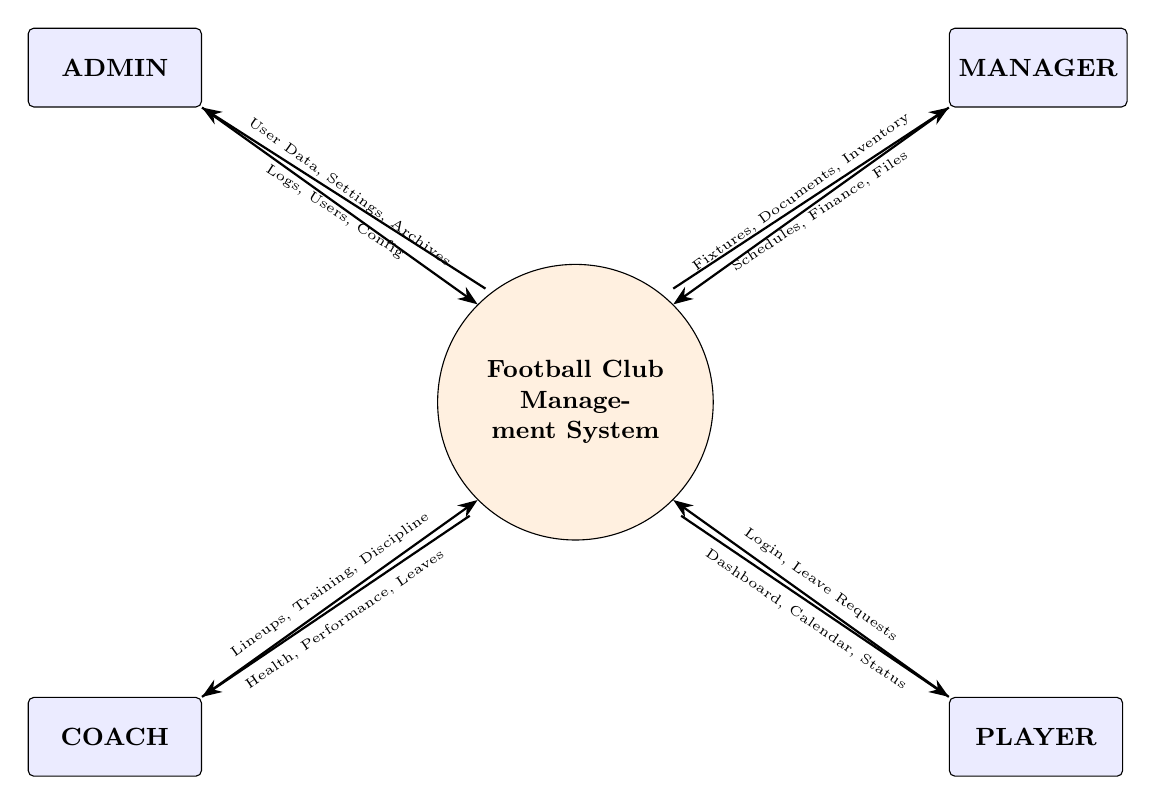
\begin{tikzpicture}[node distance=2.5cm]
  % Central system
  \node[circle, draw, fill=orange!12, minimum size=3.5cm, font=\small\bfseries, text width=2.8cm, align=center]
    (sys) {Football Club Management System};

  % External entities
  \node[entity, above left=2.5cm and 3.5cm of sys]  (admin)   {ADMIN};
  \node[entity, above right=2.5cm and 3.5cm of sys] (manager) {MANAGER};
  \node[entity, below left=2.5cm and 3.5cm of sys]  (coach)   {COACH};
  \node[entity, below right=2.5cm and 3.5cm of sys] (player)  {PLAYER};

  % Arrows — Admin
  \draw[arrow] (admin.south east) -- node[above, sloped, font=\tiny]{User Data, Settings, Archives} (sys.north west);
  \draw[arrow] (sys.north west) ++(0.1,0.2) -- node[below, sloped, font=\tiny]{Logs, Users, Config} (admin.south east);

  % Arrows — Manager
  \draw[arrow] (manager.south west) -- node[above, sloped, font=\tiny]{Fixtures, Documents, Inventory} (sys.north east);
  \draw[arrow] (sys.north east) ++(0.0,0.2) -- node[below, sloped, font=\tiny]{Schedules, Finance, Files} (manager.south west);

  % Arrows — Coach
  \draw[arrow] (coach.north east) -- node[above, sloped, font=\tiny]{Lineups, Training, Discipline} (sys.south west);
  \draw[arrow] (sys.south west) ++(-0.1,-0.2) -- node[below, sloped, font=\tiny]{Health, Performance, Leaves} (coach.north east);

  % Arrows — Player
  \draw[arrow] (player.north west) -- node[above, sloped, font=\tiny]{Login, Leave Requests} (sys.south east);
  \draw[arrow] (sys.south east) ++(0.1,-0.2) -- node[below, sloped, font=\tiny]{Dashboard, Calendar, Status} (player.north west);
\end{tikzpicture}
\caption{Level 0 --- Context Diagram}
\label{fig:dfd_l0}
\end{figure}

\subsection{Level 1 --- Admin Module DFD}

Figure~\ref{fig:dfd_admin} decomposes the Admin's interactions into sub-processes.

\begin{figure}[H]
\centering
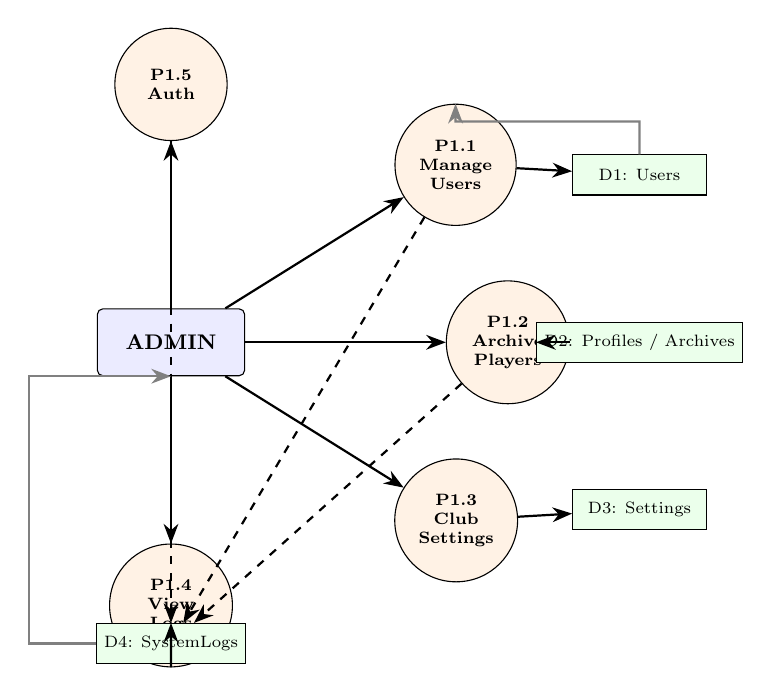
\begin{tikzpicture}[node distance=1.5cm and 2cm, scale=0.85, every node/.style={transform shape}]
  % Entity
  \node[entity] (admin) at (0,0) {ADMIN};

  % Processes
  \node[process, above right=1.5cm and 2.5cm of admin] (p1) {P1.1 Manage Users};
  \node[process, right=3cm of admin] (p2) {P1.2 Archive Players};
  \node[process, below right=1.5cm and 2.5cm of admin] (p3) {P1.3 Club Settings};
  \node[process, below=2.5cm of admin] (p4) {P1.4 View Logs};
  \node[process, above=2.5cm of admin] (p5) {P1.5 Auth};

  % Data Stores
  \node[draw, fill=green!8, minimum width=2cm, minimum height=0.6cm, font=\scriptsize] (d1) at (7,2.5) {D1: Users};
  \node[draw, fill=green!8, minimum width=2cm, minimum height=0.6cm, font=\scriptsize] (d2) at (7,0) {D2: Profiles / Archives};
  \node[draw, fill=green!8, minimum width=2cm, minimum height=0.6cm, font=\scriptsize] (d3) at (7,-2.5) {D3: Settings};
  \node[draw, fill=green!8, minimum width=2cm, minimum height=0.6cm, font=\scriptsize] (d4) at (0,-4.5) {D4: SystemLogs};

  % Arrows from Admin
  \draw[arrow] (admin) -- (p1);
  \draw[arrow] (admin) -- (p2);
  \draw[arrow] (admin) -- (p3);
  \draw[arrow] (admin) -- (p4);
  \draw[arrow] (admin) -- (p5);

  % Process to Data Store
  \draw[arrow] (p1) -- (d1);
  \draw[arrow] (p2) -- (d2);
  \draw[arrow] (p3) -- (d3);
  \draw[arrow] (p4) -- (d4);
  \draw[arrow, dashed] (p1) -- (d4);
  \draw[arrow, dashed] (p2) -- (d4);
  \draw[arrow, dashed] (p5) -- (d4);

  % Return arrows
  \draw[arrow, gray] (d1) -- ++(0,0.8) -| (p1);
  \draw[arrow, gray] (d4.west) -- ++(-1,0) |- (admin.south);
\end{tikzpicture}
\caption{Level 1 --- Admin Module DFD}
\label{fig:dfd_admin}
\end{figure}

\subsection{Level 1 --- Manager Module DFD}

Figure~\ref{fig:dfd_manager} shows the Manager's sub-processes for scheduling and resource management.

\begin{figure}[H]
\centering
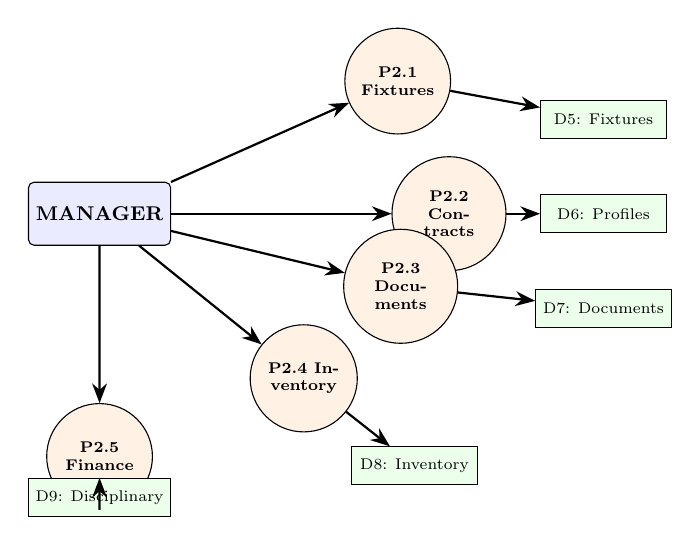
\begin{tikzpicture}[node distance=1.2cm and 2cm, scale=0.8, every node/.style={transform shape}]
  \node[entity] (mgr) at (0,0) {MANAGER};

  \node[process, above right=1cm and 3cm of mgr] (p1) {P2.1 Fixtures};
  \node[process, right=3.5cm of mgr] (p2) {P2.2 Contracts};
  \node[process, below right=0cm and 3cm of mgr] (p3) {P2.3 Documents};
  \node[process, below right=1.5cm and 1.5cm of mgr] (p4) {P2.4 Inventory};
  \node[process, below=2.5cm of mgr] (p5) {P2.5 Finance};

  \node[draw, fill=green!8, minimum width=2cm, minimum height=0.6cm, font=\scriptsize]
    (d5) at (8,1.5) {D5: Fixtures};
  \node[draw, fill=green!8, minimum width=2cm, minimum height=0.6cm, font=\scriptsize]
    (d6) at (8,0) {D6: Profiles};
  \node[draw, fill=green!8, minimum width=2cm, minimum height=0.6cm, font=\scriptsize]
    (d7) at (8,-1.5) {D7: Documents};
  \node[draw, fill=green!8, minimum width=2cm, minimum height=0.6cm, font=\scriptsize]
    (d8) at (5,-4) {D8: Inventory};
  \node[draw, fill=green!8, minimum width=2cm, minimum height=0.6cm, font=\scriptsize]
    (d9) at (0,-4.5) {D9: Disciplinary};

  \draw[arrow] (mgr) -- (p1);
  \draw[arrow] (mgr) -- (p2);
  \draw[arrow] (mgr) -- (p3);
  \draw[arrow] (mgr) -- (p4);
  \draw[arrow] (mgr) -- (p5);

  \draw[arrow] (p1) -- (d5);
  \draw[arrow] (p2) -- (d6);
  \draw[arrow] (p3) -- (d7);
  \draw[arrow] (p4) -- (d8);
  \draw[arrow] (p5) -- (d9);
\end{tikzpicture}
\caption{Level 1 --- Manager Module DFD}
\label{fig:dfd_manager}
\end{figure}

\subsection{Level 1 --- Coach Module DFD}

Figure~\ref{fig:dfd_coach} details the Coach's tactical and squad management processes.

\begin{figure}[H]
\centering
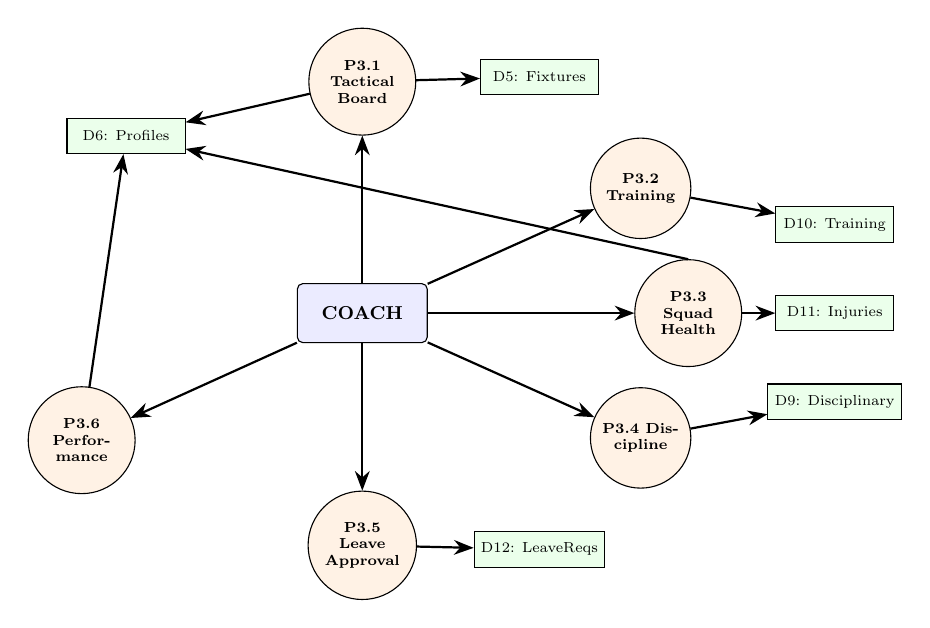
\begin{tikzpicture}[node distance=1cm and 2cm, scale=0.75, every node/.style={transform shape}]
  \node[entity] (coach) at (0,0) {COACH};

  \node[process, above=2.5cm of coach] (p1) {P3.1 Tactical Board};
  \node[process, above right=1cm and 3cm of coach] (p2) {P3.2 Training};
  \node[process, right=3.5cm of coach] (p3) {P3.3 Squad Health};
  \node[process, below right=1cm and 3cm of coach] (p4) {P3.4 Discipline};
  \node[process, below=2.5cm of coach] (p5) {P3.5 Leave Approval};
  \node[process, below left=1cm and 3cm of coach] (p6) {P3.6 Performance};

  \node[draw, fill=green!8, minimum width=2cm, minimum height=0.6cm, font=\scriptsize]
    (d5) at (3,4) {D5: Fixtures};
  \node[draw, fill=green!8, minimum width=2cm, minimum height=0.6cm, font=\scriptsize]
    (d6) at (-4,3) {D6: Profiles};
  \node[draw, fill=green!8, minimum width=2cm, minimum height=0.6cm, font=\scriptsize]
    (d10) at (8,1.5) {D10: Training};
  \node[draw, fill=green!8, minimum width=2cm, minimum height=0.6cm, font=\scriptsize]
    (d11) at (8,0) {D11: Injuries};
  \node[draw, fill=green!8, minimum width=2cm, minimum height=0.6cm, font=\scriptsize]
    (d9) at (8,-1.5) {D9: Disciplinary};
  \node[draw, fill=green!8, minimum width=2cm, minimum height=0.6cm, font=\scriptsize]
    (d12) at (3,-4) {D12: LeaveReqs};

  \draw[arrow] (coach) -- (p1);
  \draw[arrow] (coach) -- (p2);
  \draw[arrow] (coach) -- (p3);
  \draw[arrow] (coach) -- (p4);
  \draw[arrow] (coach) -- (p5);
  \draw[arrow] (coach) -- (p6);

  \draw[arrow] (p1) -- (d5);
  \draw[arrow] (p1) -- (d6);
  \draw[arrow] (p2) -- (d10);
  \draw[arrow] (p3) -- (d11);
  \draw[arrow] (p3.north) -- (d6);
  \draw[arrow] (p4) -- (d9);
  \draw[arrow] (p5) -- (d12);
  \draw[arrow] (p6) -- (d6);
\end{tikzpicture}
\caption{Level 1 --- Coach Module DFD}
\label{fig:dfd_coach}
\end{figure}

\subsection{Level 1 --- Player Module DFD}

Figure~\ref{fig:dfd_player} shows the Player's view-and-submit processes.

\begin{figure}[H]
\centering
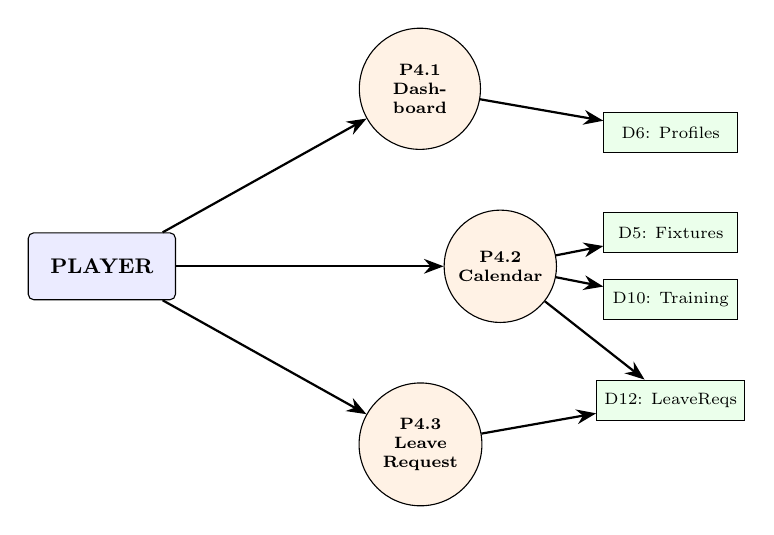
\begin{tikzpicture}[node distance=1.5cm and 2.5cm, scale=0.85, every node/.style={transform shape}]
  \node[entity] (player) at (0,0) {PLAYER};

  \node[process, above right=1.5cm and 3cm of player] (p1) {P4.1 Dashboard};
  \node[process, right=4cm of player] (p2) {P4.2 Calendar};
  \node[process, below right=1.5cm and 3cm of player] (p3) {P4.3 Leave Request};

  \node[draw, fill=green!8, minimum width=2cm, minimum height=0.6cm, font=\scriptsize]
    (d6) at (8.5,2) {D6: Profiles};
  \node[draw, fill=green!8, minimum width=2cm, minimum height=0.6cm, font=\scriptsize]
    (d5) at (8.5,0.5) {D5: Fixtures};
  \node[draw, fill=green!8, minimum width=2cm, minimum height=0.6cm, font=\scriptsize]
    (d10) at (8.5,-0.5) {D10: Training};
  \node[draw, fill=green!8, minimum width=2cm, minimum height=0.6cm, font=\scriptsize]
    (d12) at (8.5,-2) {D12: LeaveReqs};

  \draw[arrow] (player) -- (p1);
  \draw[arrow] (player) -- (p2);
  \draw[arrow] (player) -- (p3);

  \draw[arrow] (p1) -- (d6);
  \draw[arrow] (p2) -- (d5);
  \draw[arrow] (p2) -- (d10);
  \draw[arrow] (p2) -- (d12);
  \draw[arrow] (p3) -- (d12);
\end{tikzpicture}
\caption{Level 1 --- Player Module DFD}
\label{fig:dfd_player}
\end{figure}


\section{Entity Relationship Diagram}

Figure~\ref{fig:erd} illustrates the relationships among the 15 MongoDB collections.

\begin{figure}[H]
\centering
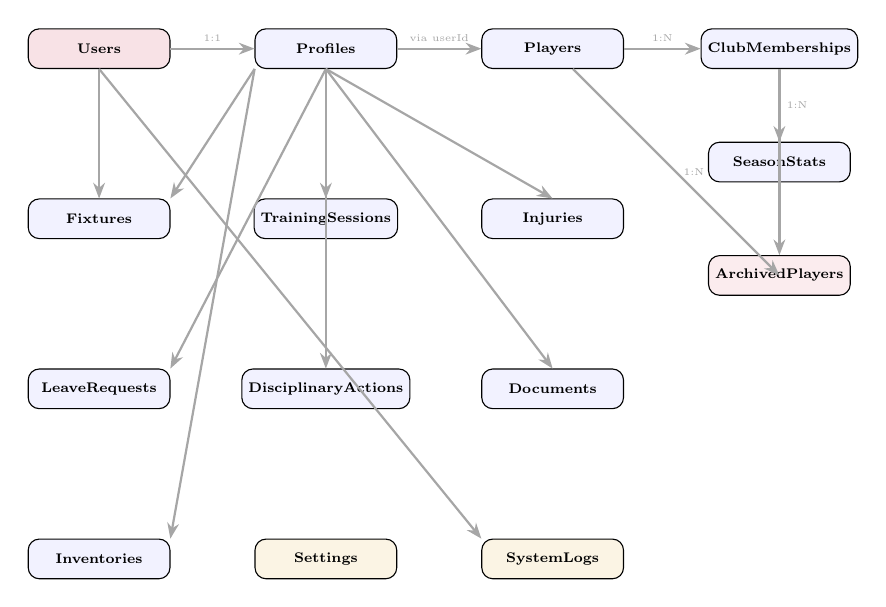
\begin{tikzpicture}[
  entity box/.style={draw, rounded corners=4pt, fill=blue!5, minimum width=2.5cm, minimum height=0.7cm, font=\scriptsize\bfseries, text centered},
  rel/.style={-{Stealth[length=2mm]}, thick, gray!70},
  scale=0.72, every node/.style={transform shape}
]
  % Core entities
  \node[entity box, fill=fcRed!12] (users) at (0,0) {Users};
  \node[entity box] (profiles) at (4,0) {Profiles};
  \node[entity box] (players) at (8,0) {Players};
  \node[entity box] (club) at (12,0) {ClubMemberships};
  \node[entity box] (season) at (12,-2) {SeasonStats};
  \node[entity box, fill=fcRed!8] (archive) at (12,-4) {ArchivedPlayers};

  \node[entity box] (fixtures) at (0,-3) {Fixtures};
  \node[entity box] (training) at (4,-3) {TrainingSessions};
  \node[entity box] (injuries) at (8,-3) {Injuries};

  \node[entity box] (leave) at (0,-6) {LeaveRequests};
  \node[entity box] (disc) at (4,-6) {DisciplinaryActions};
  \node[entity box] (docs) at (8,-6) {Documents};

  \node[entity box] (inv) at (0,-9) {Inventories};
  \node[entity box, fill=accentGold!12] (settings) at (4,-9) {Settings};
  \node[entity box, fill=accentGold!12] (logs) at (8,-9) {SystemLogs};

  % Relationships
  \draw[rel] (users) -- node[above, font=\tiny]{1:1} (profiles);
  \draw[rel] (profiles) -- node[above, font=\tiny]{via userId} (players);
  \draw[rel] (players) -- node[above, font=\tiny]{1:N} (club);
  \draw[rel] (club) -- node[right, font=\tiny]{1:N} (season);
  \draw[rel] (players) -- node[right, font=\tiny]{1:N} ++(4,-4);
  \draw[rel] (club.south) -- (archive.north);

  \draw[rel] (profiles.south) -- (training.north);
  \draw[rel] (profiles.south) -- (injuries.north);
  \draw[rel] (profiles.south west) -- (fixtures.north east);

  \draw[rel] (profiles.south) -- (leave.north east);
  \draw[rel] (profiles.south) -- (disc.north);
  \draw[rel] (profiles.south) -- (docs.north);
  \draw[rel] (profiles.south west) -- (inv.north east);

  \draw[rel] (users.south) -- (logs.north west);
  \draw[rel] (users.south) -- (fixtures.north);

\end{tikzpicture}
\caption{Entity Relationship Diagram --- 15 Collections}
\label{fig:erd}
\end{figure}


% ────────────────────────────────────────────────────────────────────────────
%  CHAPTER 5: TABLE DESIGN
% ────────────────────────────────────────────────────────────────────────────
\chapter{TABLE DESIGN}

The system uses \textbf{15 MongoDB collections} with Mongoose ODM for schema enforcement, validation, virtuals, and pre/post hooks. MongoDB uses \texttt{\_id} (ObjectId) as the auto-generated primary key for every document. The following sections detail each collection's structure.

\section{Users Collection}

\begin{table}[H]
\centering
\caption{Users Collection Schema}
\label{tab:users}
\small
\begin{tabularx}{\textwidth}{|c|l|l|l|X|}
\hline
\rowcolor{tableHeader}
\textcolor{white}{\#} & \textcolor{white}{\textbf{Field}} & \textcolor{white}{\textbf{Type}} & \textcolor{white}{\textbf{Null}} & \textcolor{white}{\textbf{Constraints}} \\
\hline
1 & \_id           & ObjectId         & NO  & Primary Key (auto) \\
\hline\rowcolor{tableRow}
2 & email          & String           & NO  & UNIQUE, lowercase, RFC~5322 regex \\
\hline
3 & passwordHash   & String           & NO  & bcrypt hashed; select:false \\
\hline\rowcolor{tableRow}
4 & role           & String (enum)    & NO  & IN: admin, manager, coach, player \\
\hline
5 & createdAt      & Date             & NO  & Immutable, default: Date.now \\
\hline
\end{tabularx}
\end{table}

\noindent\textbf{Indexes:} \texttt{\{role: 1\}}

\section{Profiles Collection}

\begin{table}[H]
\centering
\caption{Profiles Collection Schema (Key Fields)}
\label{tab:profiles}
\small
\begin{tabularx}{\textwidth}{|c|l|l|l|X|}
\hline
\rowcolor{tableHeader}
\textcolor{white}{\#} & \textcolor{white}{\textbf{Field}} & \textcolor{white}{\textbf{Type}} & \textcolor{white}{\textbf{Null}} & \textcolor{white}{\textbf{Constraints}} \\
\hline
1 & userId            & ObjectId (ref: User)  & NO  & UNIQUE, FK to Users \\
\hline\rowcolor{tableRow}
2 & fullName          & String                & NO  & 2--100 chars \\
\hline
3 & position          & String (enum)         & YES & GK, DEF, MID, FWD, Staff \\
\hline\rowcolor{tableRow}
4 & fitnessStatus     & String (enum)         & YES & Green, Yellow, Red \\
\hline
5 & contractType      & String (enum)         & YES & Full-Time, Part-Time, Loan, Trial \\
\hline\rowcolor{tableRow}
6 & contractStart     & Date                  & YES & --- \\
\hline
7 & contractEnd       & Date                  & YES & Must be $\geq$ contractStart \\
\hline\rowcolor{tableRow}
8 & stats.*           & Number (sub-doc)      & YES & goals, assists, appearances, rating, etc. \\
\hline
9 & performanceNotes  & Array of Sub-doc      & YES & note, createdBy, createdAt \\
\hline
\end{tabularx}
\end{table}

\noindent\textbf{Indexes:} \texttt{\{fitnessStatus: 1\}}, \texttt{\{contractEnd: 1\}}\\
\textbf{Virtuals:} \texttt{contractDaysRemaining}, \texttt{contractExpiringSoon} ($<90$ days)

\section{Players Collection}

\begin{table}[H]
\centering
\caption{Players Collection Schema}
\label{tab:players}
\small
\begin{tabularx}{\textwidth}{|c|l|l|l|X|}
\hline
\rowcolor{tableHeader}
\textcolor{white}{\#} & \textcolor{white}{\textbf{Field}} & \textcolor{white}{\textbf{Type}} & \textcolor{white}{\textbf{Null}} & \textcolor{white}{\textbf{Constraints}} \\
\hline
1 & fullName       & String            & NO  & 2--100 chars \\
\hline\rowcolor{tableRow}
2 & dateOfBirth    & Date              & YES & --- \\
\hline
3 & nationality    & String            & YES & Max 60 chars \\
\hline\rowcolor{tableRow}
4 & status         & String (enum)     & YES & active, archived, transferred, retired \\
\hline
5 & currentUserId  & ObjectId (ref)    & YES & Sparse index \\
\hline
\end{tabularx}
\end{table}

\section{ClubMemberships Collection}

Tracks a player's tenure, jersey number, position, contract, and availability. Key fields include \texttt{playerId} (FK to Players), \texttt{jerseyNumber} (1--99), \texttt{primaryPosition}, \texttt{contractType} (Owned/Loan/Academy/Trial/Staff), \texttt{squadRole} (starter/rotation/prospect/captain), and \texttt{availabilityStatus} with detail sub-document.

\noindent\textbf{Indexes:} \texttt{\{playerId:1, isActive:1\}}, \texttt{\{jerseyNumber:1, isActive:1\}}, \texttt{\{joinedAt:-1\}}

\section{SeasonStats Collection}

Stores per-season statistics: goals, assists, yellowCards, redCards, minutesPlayed, appearances, offsides, and matchRatings (array of fixture-specific ratings with coach notes). Compound unique index on \texttt{\{membershipId, season\}}.

\noindent\textbf{Virtuals:} \texttt{averageRating} computed from matchRatings array.

\section{ArchivedPlayers Collection}

Preserves a frozen snapshot of a player upon archival. Contains \texttt{reason} (transferred/released/retired/etc.), \texttt{careerSummaryAtClub} (totalGoals, totalAssists, totalAppearances, seasonsPlayed, trophiesWon), and \texttt{snapshot} (fullName, photo, jerseyNumber, position at time of archival).

\section{Fixtures Collection}

\begin{table}[H]
\centering
\caption{Fixtures Collection Schema}
\label{tab:fixtures}
\small
\begin{tabularx}{\textwidth}{|c|l|l|l|X|}
\hline
\rowcolor{tableHeader}
\textcolor{white}{\#} & \textcolor{white}{\textbf{Field}} & \textcolor{white}{\textbf{Type}} & \textcolor{white}{\textbf{Null}} & \textcolor{white}{\textbf{Constraints}} \\
\hline
1 & opponent        & String                & NO  & 2--100 chars \\
\hline\rowcolor{tableRow}
2 & date            & Date                  & NO  & Cannot be in the past \\
\hline
3 & location        & String                & NO  & --- \\
\hline\rowcolor{tableRow}
4 & matchType       & String (enum)         & YES & League, Cup, Friendly, Tournament \\
\hline
5 & lineup          & Array of ObjectId     & YES & Max 18 (11 starters + 7 subs) \\
\hline\rowcolor{tableRow}
6 & lineupHistory   & Array of Sub-doc      & YES & version, savedAt, savedBy, formation \\
\hline
\end{tabularx}
\end{table}

\section{TrainingSessions Collection}

Fields: \texttt{date} (future only), \texttt{drillDescription} (10--500 chars), \texttt{duration} (30--300 min), \texttt{attendees} (array of sub-docs with playerId and status: Present/Absent/Excused), \texttt{createdBy}.

\section{Injuries Collection}

Fields: \texttt{playerId} (FK), \texttt{injuryType}, \texttt{severity} (Minor/Moderate/Severe), \texttt{expectedRecovery}, \texttt{resolved} (boolean), \texttt{loggedBy}.

\section{LeaveRequests Collection}

Fields: \texttt{playerId}, \texttt{startDate}, \texttt{endDate} ($\geq$ startDate), \texttt{reason} (10--500 chars), \texttt{status} (Pending/Approved/Denied), \texttt{reviewedBy}, \texttt{reviewedAt}.

\section{DisciplinaryActions Collection}

Fields: \texttt{playerId}, \texttt{offense} (5--200 chars), \texttt{fineAmount} (0--100,000), \texttt{isPaid}, \texttt{paymentDate}, \texttt{issuedBy}.

\section{Documents Collection}

Fields: \texttt{playerId}, \texttt{fileName}, \texttt{originalName}, \texttt{filePath}, \texttt{fileType} (PDF/JPEG/PNG), \texttt{fileSize} (max 10~MB), \texttt{uploadedBy}.

\section{Inventories Collection}

Fields: \texttt{itemName}, \texttt{itemType} (Jersey/Boots/Training Equipment/Medical/Other), \texttt{assignedTo} (ref), \texttt{assignedAt}, \texttt{returnedAt}. Virtual: \texttt{isAssigned}.

\section{Settings Collection (Singleton)}

A single document storing: \texttt{clubName}, \texttt{logoUrl}, \texttt{homepageHeadline}, \texttt{clubDescription}, \texttt{founded}, \texttt{ground}, \texttt{league}, \texttt{contactEmail}, \texttt{socialHandle}, \texttt{trophies[]} (title+year). Uses \texttt{getSingleton()} static method.

\section{SystemLogs Collection (Immutable)}

Fields: \texttt{action} (CREATE/UPDATE/DELETE/LOGIN), \texttt{performedBy} (FK), \texttt{targetCollection}, \texttt{targetId}, \texttt{changes} (Mixed), \texttt{timestamp} (immutable). Pre-hooks prevent all update and delete operations---logs are write-once, read-many.


% ────────────────────────────────────────────────────────────────────────────
%  CHAPTER 6: MODULE DESIGN & IMPLEMENTATION
% ────────────────────────────────────────────────────────────────────────────
\chapter{MODULE DESIGN AND IMPLEMENTATION}

The system consists of four role-based modules, a shared login page, and four AI-powered features. Each module is implemented as a React page component rendered within the \texttt{PanelShell} layout---a scrollable, single-page workspace with fixed side navigation, scroll-spy highlighting, and smooth section navigation.

\section{Login Page}

The Login Page is the gateway to the system. It features a full-screen, dark-themed layout with a centered glassmorphic card containing:

\begin{itemize}[leftmargin=*]
  \item Club crest badge with pulsing glow animation
  \item Email and password input fields with focus-state red border transitions
  \item ``SIGN IN'' button with hover lift effect and loading state
  \item Error alert banner for failed authentication
\end{itemize}

\noindent\textbf{Authentication Flow:} User submits credentials $\rightarrow$ AuthContext sends POST to \texttt{/api/auth/login} $\rightarrow$ Backend validates via bcrypt, generates JWT $\rightarrow$ SystemLog records LOGIN event $\rightarrow$ Frontend stores token, redirects to role-specific panel. Token verification runs on every page mount via \texttt{GET /api/auth/verify}.

\section{Admin Module}

Route: \texttt{/admin} \quad Allowed Role: admin only

\subsection{User Management}
Full CRUD capabilities for all user accounts (admin, manager, coach, player) displayed in a table/grid format. Features inline creation form with email validation, role selector, and bcrypt-hashed password storage. Every mutation is logged to SystemLogs.

\subsection{Player Archive}
Manages the complete player lifecycle. Administrators can archive players with reason selection (transferred/released/retired/etc.) and notes, view archived players with frozen career snapshots (totalGoals, totalAssists, totalAppearances), and reinstate archived players.

\subsection{Club Settings}
Manages club identity through a singleton Settings document: club name, logo, headline, description, founded year, stadium, league, contact email, social handle, and dynamic trophies list.

\subsection{System Logs}
Read-only immutable audit trail with filter bar (action type, collection, date range, performer), chronologically sorted log table with color-coded action badges, and live presence indicator via Socket.IO.

\section{Manager Module}

Route: \texttt{/manager} \quad Allowed Role: manager only

\subsection{Fixtures}
Fixture scheduling with opponent, date (future-only validation), location, and match type. Cards display upcoming and past fixtures.

\subsection{Contracts}
Contract lifecycle tracking with overview grid showing contract type, start/end dates, days remaining, and red-highlighted expiry alerts for contracts expiring within 90 days.

\subsection{Document Vault}
Secure file management with drag-and-drop upload (PDF/JPEG/PNG, max 10~MB), document grid with metadata, download links, and OCR scanner integration for text extraction.

\subsection{Inventory}
Equipment tracking with item creation, player assignment/return workflows, and status badges (Assigned/Available). Virtual \texttt{isAssigned} computed from assignment state.

\subsection{Finance Dashboard}
Disciplinary fine tracking with summary cards (total/paid/unpaid fines, payment rate), detailed fine table, and mark-as-paid functionality.

\section{Coach Module}

Route: \texttt{/coach} \quad Allowed Role: coach only

\subsection{Tactical Board}
The largest and most complex component. Features fixture selector, formation dropdown (4-3-3, 4-4-2, 3-5-2, etc.), CSS-drawn pitch visualization with drag-and-drop player tokens (11 starters + 7 subs), player pool with position and fitness filters, lineup validation (max 18), and version history.

\subsection{Training Schedule}
Session creation with date, drill description (10--500 chars), duration (30--300 min), and per-player attendance marking (Present/Absent/Excused) with bulk capabilities.

\subsection{Squad Health}
Color-coded fitness overview (Green/Yellow/Red), injury logging with severity levels, injury history with resolution tracking, and manual availability override.

\subsection{Discipline}
Disciplinary action management with fine issuance (offense + amount), payment status tracking, and payment toggle.

\subsection{Leave Approval}
Pending request cards with Approve/Deny buttons and request history with status badges. Approval triggers real-time Socket.IO notification to the player.

\subsection{Performance Tracking}
Stat editor for goals, assists, appearances, minutes, cards, and rating (0--10). Performance notes timeline with coach attribution and timestamps.

\section{Player Module}

Route: \texttt{/player} \quad Allowed Role: player only

\subsection{Personalized Dashboard}
Landing page with profile header, statistics grid (goals, assists, appearances, rating), contract information with expiry countdown, recent performance notes, and EA~FC-style animated player card.

\subsection{Calendar}
Unified monthly calendar combining fixtures, training sessions, and approved leave dates with color-coded legend (Matches=red, Training=blue, Leave=green).

\subsection{Leave Requests}
Submit form with date pickers and reason textarea (10--500 chars). Request history shows status badges and review details.

\section{AI-Powered Features}

\subsection{OCR Document Scanner}
Extracts text from uploaded documents (PDF/image) for searching and indexing. Multi-page PDF support.

\subsection{AI Document Preparation}
Auto-generates standardized club documents from templates pre-filled with player data from multiple collections.

\subsection{AI Chatbot}
Natural language query interface accessible from any panel. Maps questions to database queries and returns human-readable responses.

\subsection{Text Summarization}
Condenses long document text into concise bullet-point summaries highlighting key facts, dates, and numbers.


% ────────────────────────────────────────────────────────────────────────────
%  CHAPTER 7: SECURITY
% ────────────────────────────────────────────────────────────────────────────
\chapter{SECURITY MEASURES}

The system implements a multi-layered security architecture. Table~\ref{tab:security} summarizes all 17 security features.

\begin{longtable}{|c|p{3.2cm}|p{3cm}|p{5.5cm}|}
\caption{Security Features Summary}
\label{tab:security} \\
\hline
\rowcolor{tableHeader}
\textcolor{white}{\#} & \textcolor{white}{\textbf{Feature}} & \textcolor{white}{\textbf{Technology}} & \textcolor{white}{\textbf{Description}} \\
\hline
\endfirsthead
\hline
\rowcolor{tableHeader}
\textcolor{white}{\#} & \textcolor{white}{\textbf{Feature}} & \textcolor{white}{\textbf{Technology}} & \textcolor{white}{\textbf{Description}} \\
\hline
\endhead
1  & JWT Authentication     & jsonwebtoken v9.0.2   & Bearer token in every request; contains \{id, role\} payload \\
\hline\rowcolor{tableRow}
2  & Password Hashing       & bcrypt v5.1.1         & Salt rounds=10; select:false excludes hash from queries \\
\hline
3  & RBAC                   & roleGuard middleware   & requireRole() restricts routes to specific roles; returns 403 \\
\hline\rowcolor{tableRow}
4  & Frontend Protection    & ProtectedRoute.jsx    & Redirects unauthorized users to login \\
\hline
5  & Security Headers       & Helmet v7.1.0         & CSP, X-Frame-Options, HSTS, X-Content-Type-Options \\
\hline\rowcolor{tableRow}
6  & CORS Policy            & cors v2.8.5           & Restricted to specific client URL; credentials enabled \\
\hline
7  & Rate Limiting          & express-rate-limit    & API: 100/15min; Auth: 5/15min; Uploads: 10/15min \\
\hline\rowcolor{tableRow}
8  & Input Sanitization     & sanitize-html + validator & XSS prevention; RFC 5322 email validation \\
\hline
9  & Schema Validation      & Mongoose validators   & Type, min/max, enum, custom validators; 400 on failure \\
\hline\rowcolor{tableRow}
10 & Immutable Audit Logs   & SystemLog pre-hooks   & Prevents UPDATE/DELETE; write-once, read-many \\
\hline
11 & Password Exclusion     & select:false + transform & Hash never in query results or serialized output \\
\hline\rowcolor{tableRow}
12 & Compression            & compression v1.7.4    & Gzip-compressed API responses \\
\hline
13 & Env Variable Security  & dotenv v16.3.1        & Secrets in git-ignored .env files \\
\hline\rowcolor{tableRow}
14 & File Upload Validation & Multer config         & PDF/JPEG/PNG only; max 10~MB \\
\hline
15 & Global Error Handler   & errorHandler.js       & Type-specific handling; stack traces only in dev \\
\hline\rowcolor{tableRow}
16 & Socket.IO Auth         & JWT on connection     & WebSocket connections require valid tokens \\
\hline
17 & 404 Handler            & notFoundHandler       & Structured error; prevents info leakage \\
\hline
\end{longtable}


% ────────────────────────────────────────────────────────────────────────────
%  CHAPTER 8: SYSTEM TESTING
% ────────────────────────────────────────────────────────────────────────────
\chapter{SYSTEM TESTING}

\section{Unit Testing}

Unit testing was performed using \textbf{Jest v29.7.0} with \textbf{fast-check v3.15.0} for property-based testing. Tests verify individual components in isolation:

\begin{itemize}[leftmargin=*]
  \item \textbf{Model Tests:} Valid document creation, validation failures, virtual computation, immutability enforcement, and pre-hook behavior for each Mongoose model.
  \item \textbf{Controller Tests:} Correct HTTP status codes, response body structure, database interaction, and edge-case error handling.
  \item \textbf{Middleware Tests:} Token validation, role-based access, rate limiting, and error formatting.
  \item \textbf{Frontend Tests:} Component rendering, state management, form validation, and animation states.
\end{itemize}

\section{Integration Testing}

Integration testing used \textbf{Jest + Supertest v6.3.3} to verify end-to-end flows:

\begin{itemize}[leftmargin=*]
  \item \textbf{API Channel:} Client sends request with JWT $\rightarrow$ Express processes $\rightarrow$ Mongoose queries MongoDB $\rightarrow$ JSON response returned. Verified CRUD operations generate corresponding SystemLog entries.
  \item \textbf{Real-Time Channel:} Player submits leave request $\rightarrow$ API saves to database $\rightarrow$ Socket.IO pushes notification to Coach $\rightarrow$ Coach approves $\rightarrow$ Player receives instant status update---all without page refresh.
\end{itemize}

\section{Test Cases}

Table~\ref{tab:testcases} documents the 25 formal test cases.

\begin{longtable}{|l|l|p{4.5cm}|p{4.5cm}|c|}
\caption{System Test Cases}
\label{tab:testcases} \\
\hline
\rowcolor{tableHeader}
\textcolor{white}{\textbf{ID}} & \textcolor{white}{\textbf{Module}} & \textcolor{white}{\textbf{Test Case}} & \textcolor{white}{\textbf{Expected Result}} & \textcolor{white}{\textbf{Status}} \\
\hline
\endfirsthead
\hline
\rowcolor{tableHeader}
\textcolor{white}{\textbf{ID}} & \textcolor{white}{\textbf{Module}} & \textcolor{white}{\textbf{Test Case}} & \textcolor{white}{\textbf{Expected Result}} & \textcolor{white}{\textbf{Status}} \\
\hline
\endhead
TC-001 & Auth    & Valid login          & 200, JWT + role            & Pass \\
\hline\rowcolor{tableRow}
TC-002 & Auth    & Invalid password     & 401, Invalid credentials   & Pass \\
\hline
TC-003 & Auth    & Non-existent email   & 401, Auth failed           & Pass \\
\hline\rowcolor{tableRow}
TC-004 & Auth    & Empty fields         & 400, Required fields       & Pass \\
\hline
TC-005 & Auth    & No token             & 401, No auth header        & Pass \\
\hline\rowcolor{tableRow}
TC-006 & Auth    & Expired token        & 401, Token expired         & Pass \\
\hline
TC-007 & Auth    & Wrong role access    & 403, Access denied         & Pass \\
\hline\rowcolor{tableRow}
TC-008 & Admin   & Create valid user    & 201, user object           & Pass \\
\hline
TC-009 & Admin   & Duplicate email      & 400, Duplicate email       & Pass \\
\hline\rowcolor{tableRow}
TC-010 & Admin   & Invalid role         & 400, Invalid role          & Pass \\
\hline
TC-011 & Manager & Past-date fixture    & 400, Cannot be past        & Pass \\
\hline\rowcolor{tableRow}
TC-012 & Manager & Valid fixture        & 201, fixture object        & Pass \\
\hline
TC-013 & Manager & Oversize upload      & 400, Size exceeds max      & Pass \\
\hline\rowcolor{tableRow}
TC-014 & Manager & Invalid file type    & 400, Invalid type          & Pass \\
\hline
TC-015 & Coach   & Lineup $>$ 18       & 400, Max 18 exceeded       & Pass \\
\hline\rowcolor{tableRow}
TC-016 & Coach   & Training $<$ 30 min & 400, Min 30 minutes        & Pass \\
\hline
TC-017 & Coach   & Invalid severity     & 400, Not valid severity    & Pass \\
\hline\rowcolor{tableRow}
TC-018 & Coach   & Approve leave        & 200, Updated request       & Pass \\
\hline
TC-019 & Player  & End before start     & 400, End $\geq$ start     & Pass \\
\hline\rowcolor{tableRow}
TC-020 & Player  & Short reason         & 400, Min 10 chars          & Pass \\
\hline
TC-021 & Security& Modify SystemLog     & 500, Cannot modify         & Pass \\
\hline\rowcolor{tableRow}
TC-022 & Security& Delete SystemLog     & 500, Cannot delete         & Pass \\
\hline
TC-023 & Security& Rate limit           & 429, Too many attempts     & Pass \\
\hline\rowcolor{tableRow}
TC-024 & Settings& Short club name      & 400, Min 3 chars           & Pass \\
\hline
TC-025 & Profile & Invalid contract     & 400, End after start       & Pass \\
\hline
\end{longtable}

\section{User Acceptance Testing}

UAT was conducted with representative users from each role. Table~\ref{tab:uat} summarizes the results.

\begin{longtable}{|l|l|p{4cm}|p{4.5cm}|c|}
\caption{User Acceptance Testing Results}
\label{tab:uat} \\
\hline
\rowcolor{tableHeader}
\textcolor{white}{\textbf{ID}} & \textcolor{white}{\textbf{Role}} & \textcolor{white}{\textbf{Scenario}} & \textcolor{white}{\textbf{Acceptance Criteria}} & \textcolor{white}{\textbf{Result}} \\
\hline
\endfirsthead
\hline
\rowcolor{tableHeader}
\textcolor{white}{\textbf{ID}} & \textcolor{white}{\textbf{Role}} & \textcolor{white}{\textbf{Scenario}} & \textcolor{white}{\textbf{Acceptance Criteria}} & \textcolor{white}{\textbf{Result}} \\
\hline
\endhead
UAT-01  & Admin   & Create player account     & User in list with correct role    & Accepted \\
\hline\rowcolor{tableRow}
UAT-02  & Admin   & Archive retired player    & Career summary preserved          & Accepted \\
\hline
UAT-03  & Admin   & Update club identity      & Homepage reflects changes          & Accepted \\
\hline\rowcolor{tableRow}
UAT-04  & Admin   & Review audit logs         & Login events with timestamps       & Accepted \\
\hline
UAT-05  & Manager & Schedule league match     & Fixture appears for all roles      & Accepted \\
\hline\rowcolor{tableRow}
UAT-06  & Manager & Upload contract PDF       & Document in vault with metadata    & Accepted \\
\hline
UAT-07  & Manager & Assign jersey             & Inventory shows assignment         & Accepted \\
\hline\rowcolor{tableRow}
UAT-08  & Manager & View financial summary    & Totals match fine records           & Accepted \\
\hline
UAT-09  & Coach   & Build 4-3-3 lineup        & 11 starters, 7 subs on pitch       & Accepted \\
\hline\rowcolor{tableRow}
UAT-10  & Coach   & Training + attendance     & Percentages correct                 & Accepted \\
\hline
UAT-11  & Coach   & Log knee injury           & Fitness status changes              & Accepted \\
\hline\rowcolor{tableRow}
UAT-12  & Coach   & Approve leave request     & Player sees Approved status         & Accepted \\
\hline
UAT-13  & Player  & View dashboard            & All stats and info correct          & Accepted \\
\hline\rowcolor{tableRow}
UAT-14  & Player  & Submit leave request      & Appears in coach's queue            & Accepted \\
\hline
UAT-15  & Player  & View calendar             & Events on correct dates             & Accepted \\
\hline
\end{longtable}


% ────────────────────────────────────────────────────────────────────────────
%  CHAPTER 9: FUTURE ENHANCEMENTS
% ────────────────────────────────────────────────────────────────────────────
\chapter{SCOPE FOR FUTURE ENHANCEMENT}

The modular MERN-stack architecture with Socket.IO real-time communication is inherently scalable. The following high-value enhancements have been identified:

\begin{enumerate}[leftmargin=*]
  \item \textbf{Mobile Application} --- A React Native app mirroring the web platform for on-the-go access.
  \item \textbf{Advanced AI Analytics} --- Machine learning for player performance prediction, injury risk assessment, and optimal lineup recommendation.
  \item \textbf{Video Analysis Integration} --- AI-powered match highlight extraction, heatmap generation, and movement tracking.
  \item \textbf{Multi-Club / Multi-Season Support} --- Managing multiple clubs with season-based data partitioning.
  \item \textbf{Financial Module Expansion} --- Salary management, transfer fees, sponsorship revenue, and full accounting.
  \item \textbf{Biometric Integration} --- Wearable device data (GPS, heart rate) feeding into the health module.
  \item \textbf{Parent/Guardian Portal} --- Limited-access view for youth academy player guardians.
  \item \textbf{Multi-Language Support (i18n)} --- Internationalization for diverse club demographics.
  \item \textbf{Progressive Web App (PWA)} --- Offline caching, push notifications, home screen installation.
  \item \textbf{Third-Party API Integrations} --- Automatic fixture imports, live scores, and league standings.
\end{enumerate}


% ────────────────────────────────────────────────────────────────────────────
%  CHAPTER 10: CONCLUSION
% ────────────────────────────────────────────────────────────────────────────
\chapter{CONCLUSION}

The Football Club Management System was undertaken to solve the deep-seated inefficiencies inherent in traditional, spreadsheet-and-paper-based football club management. The project successfully delivered a centralized, web-based digital ecosystem comprising four interconnected modules---Admin Panel, Manager Panel, Coach Panel, and Player Panel---each providing role-specific tools built on the robust MERN stack.

The system's design achieves both functional completeness and technical excellence. A secure Node.js/Express API handles all business logic with JWT authentication and bcrypt password hashing. Socket.IO provides real-time WebSocket communication for instant notifications, online presence tracking, and live data synchronization. MongoDB with Mongoose ODM serves as the single source of truth across 15 structured collections.

Key achievements include the visual \textbf{Tactical Board} with drag-and-drop lineup building and version history; the \textbf{Squad Health Monitor} with color-coded fitness indicators; the EA~FC-style \textbf{Animated Player Card} providing a cinematic digital identity; and the \textbf{Immutable Audit Trail} ensuring complete accountability.

The four AI-powered features---OCR scanning, chatbot, document preparation, and summarization---elevate the system beyond standard CRUD operations into a decision-support platform. Enterprise-grade security with 17 implemented measures protects all sensitive club data.

The system was validated through unit, integration, and user acceptance testing, with all 25 formal test cases passing successfully. The modular architecture provides a solid foundation for the future enhancements detailed in Chapter~9. In conclusion, the Football Club Management System is a comprehensive and successful project that effectively digitizes core club operations, enhances communication, ensures accountability, and delivers a premium user experience for all stakeholders.


% ────────────────────────────────────────────────────────────────────────────
%  BIBLIOGRAPHY
% ────────────────────────────────────────────────────────────────────────────
\begin{thebibliography}{99}

\bibitem{pressman}
R.~S. Pressman and B.~R. Maxim, \textit{Software Engineering: A Practitioner's Approach}, 9th~ed. McGraw-Hill Education, 2020.

\bibitem{sommerville}
I.~Sommerville, \textit{Software Engineering}, 10th~ed. Pearson Education, 2016.

\bibitem{elmasri}
R.~Elmasri and S.~B. Navathe, \textit{Fundamentals of Database Systems}, 7th~ed. Pearson Education, 2016.

\bibitem{satzinger}
J.~W. Satzinger, R.~B. Jackson, and S.~D. Burd, \textit{Systems Analysis and Design in a Changing World}, 7th~ed. Cengage Learning, 2016.

\bibitem{martin}
R.~C. Martin, \textit{Clean Architecture: A Craftsman's Guide to Software Structure and Design}. Prentice Hall, 2017.

\bibitem{richardson}
L.~Richardson and S.~Ruby, \textit{RESTful Web Services}. O'Reilly Media, 2007.

\bibitem{nodejs}
OpenJS Foundation, ``Node.js Documentation.'' [Online]. Available: \url{https://nodejs.org/docs/latest/api/}. [Accessed: Apr.~2026].

\bibitem{mongodb}
MongoDB, Inc., ``MongoDB Manual.'' [Online]. Available: \url{https://www.mongodb.com/docs/manual/}. [Accessed: Apr.~2026].

\bibitem{express}
Express.js, ``Express 4.x API Reference.'' [Online]. Available: \url{https://expressjs.com/en/4x/api.html}. [Accessed: Apr.~2026].

\bibitem{react}
Meta Platforms, Inc., ``React Documentation.'' [Online]. Available: \url{https://react.dev/}. [Accessed: Apr.~2026].

\bibitem{mongoose}
Automattic, Inc., ``Mongoose ODM Documentation.'' [Online]. Available: \url{https://mongoosejs.com/docs/}. [Accessed: Apr.~2026].

\bibitem{jwt}
M.~Jones, J.~Bradley, and N.~Sakimura, ``JSON Web Token (JWT),'' RFC~7519, May 2015. [Online]. Available: \url{https://tools.ietf.org/html/rfc7519}.

\bibitem{socketio}
Socket.IO, ``Socket.IO Documentation (v4).'' [Online]. Available: \url{https://socket.io/docs/v4/}. [Accessed: Apr.~2026].

\bibitem{owasp}
OWASP Foundation, ``OWASP Top Ten Web Application Security Risks.'' [Online]. Available: \url{https://owasp.org/www-project-top-ten/}. [Accessed: Apr.~2026].

\bibitem{vankerckhoven}
S.~Van Kerckhoven, \textit{Professional Football Club Management: Leadership for Commercial Success}. Routledge, 2020.

\end{thebibliography}

\end{document}
